\documentclass[a4paper,10pt]{report}\input{../0.Préambule/Préambule_cours_prof}\input{0_Préambule_Analyse}\begin{document}

\newpage
\setcounter{chapter}{17}
\hypertarget{Fonction de reference}{}
\chapter{Fonction de référence}

\paragraph*{Objectif du chapitre :}
\begin{enumerate}
\item[•] Construire la représentation graphique de ces fonctions
\item[•] Connaitre et utiliser le tableau de variation de ces fonctions
\item[•] Connaitre et utiliser le tableau de signe de ces fonctions
\end{enumerate}

\vspace{-5mm}
\section{Fonction carrée}

\vspace{-5mm}
\noindent \begin{minipage}{11cm}
\begin{dft}
La fonction définie sur $\R$ par $x\longmapsto x^2$ s'appelle la \textbf{fonction carrée}.
\end{dft}
\begin{center}
\begin{tikzpicture}
\tkzTabInit{$x$/0.9,$x^2$/1.7}
{$-\infty$,$0$,$+\infty$}
%\tkzTabLine{d,-,z,+}
\tkzTabVar{+/$\textcolor{lightgray}{+\infty}$,-/$0$,+/$\textcolor{lightgray}{+\infty}$}
\end{tikzpicture}
\end{center}
\end{minipage}
\begin{minipage}{6cm}
\begin{center}
\begin{tikzpicture}[line cap=round,line join=round,>=triangle 45,x=1.0cm,y=1.0cm,scale=1]
\begin{axis}[x=1.0cm,y=1.0cm,axis lines=middle,ymajorgrids=true,xmajorgrids=true,
xmin=-2.4,xmax=2.4,ymin=-1.2,ymax=3.2,xtick={-2.0,-1.0,...,2.0},ytick={-1,0,...,3.0},]
\clip(-2.4,-1.2) rectangle (2.4,3.2);
\draw[line width=2.4pt,color=blue,smooth,samples=100,domain=-2.4:2.4] plot(\x,{(\x)^(2.0)});
\begin{scriptsize}
\draw[color=blue] (2,1) node {\large{$\mathcal{C}_f$}};
\end{scriptsize}
\end{axis}
\end{tikzpicture}   
\end{center}
\end{minipage}

\medskip
\noindent Dans un repère $\Rep$, la courbe représentative de la fonction carré est une \textbf{parabole} de sommet $O$.

\noindent Cette parabole admet l'axe des ordonnées comme axe de symétrie, ce qui caractérise une fonction \textbf{paire}.

\begin{prop}
La fonction carrée est strictement décroissante sur $\Intg{-\infty}{0}$ et strictement croissante sur $\Intd{0}{+\infty}$.
\end{prop}

\begin{demoe}
Proposition à démontrer : \og La fonction carrée est strictement décroissante sur $\Intg{-\infty}{0}$ et strictement croissante sur $\Intd{0}{+\infty}$. \fg{} 

\medskip
On va faire un raisonnement par disjonction des cas :
\begin{enumerate}
\item[•]Commençons par démontrer que la fonction carrée est strictement croissante sur $\Intd{0}{+\infty}$

\medskip
Soient $a$ et $b$ deux nombres réels positifs tels que $a<b$ et la fonction $f$ définie sur $\R$ par $f(x)=x^2$
\begin{align*}
a<b \quad &\Longrightarrow \quad a \times a < b \times a \quad \text{et}\quad a \times b < b \times b\\
&\Longrightarrow \quad (a)^2 < b \times a < (b)^2 \quad \Longrightarrow \quad (a)^2 < (b)^2 \quad \Longrightarrow \quad f(a) < f(b)
\end{align*} 
Donc la fonction $f$ est strictement croissante sur $\Intd{0}{+\infty}$
%\item[•]Démontrons maintenant que la fonction carrée est strictement décroissante sur $\Intg{-\infty}{0}$

%\medskip
%Soient $x_1$ et $x_2$ deux nombres réels négatifs tels que $x_1<x_2$ et la fonction $f$ définie sur $\R$ par $f(x)=x^2$
%\begin{align*}
%a<b \quad &\Longrightarrow \quad x_1 \times a > b \times a \quad \text{et}\quad a \times b > b \times b &\text{ car } a \text{ et } b \text{ sont négatifs}\\
%&\Longrightarrow \quad (a)^2 > b \times a > (b)^2 \quad \Longrightarrow \quad (a)^2 > (b)^2 \quad \Longrightarrow \quad f(a) > f(b)
%\end{align*} 
%Donc la fonction $f$ est strictement décroissante sur $\Intg{-\infty}{0}$\hfill $\blacksquare$
\item[•] On procède de même pour montrer que la fonction carrée est strictement décroissante sur $\Intg{-\infty}{0}$ \hfill $\blacksquare$
\end{enumerate}
\end{demoe}

\vspace{-5mm}
\section{Fonction inverse}

\vspace{-5mm}
\noindent \begin{minipage}{12.5cm}
\begin{dft}
La fonction définie sur $] \, -\infty \, ; \, 0 \, [ \cup ] \, 0 \, ; \, +\infty \, [$ par $x\longmapsto \dfrac{1}{x}$ est la \textbf{fonction inverse}.
\end{dft}
\begin{center}
\begin{tikzpicture}
\tkzTabInit{$x$/1,$\dfrac{1}{x}$/1.6}
{$-\infty$,$0$,$+\infty$}
%\tkzTabLine{d,-,z,+}
\tkzTabVar{+/$$\textcolor{lightgray}{0}$$,-D+/$\textcolor{lightgray}{-\infty}$/$\textcolor{lightgray}{+\infty}$,-/$$\textcolor{lightgray}{0}$$}
\end{tikzpicture}
\end{center}
\end{minipage}
\begin{minipage}{4.5cm}
\begin{center}
\begin{tikzpicture}[line cap=round,line join=round,>=triangle 45,x=1.0cm,y=1.0cm,scale=0.65]
\begin{axis}[x=1.0cm,y=1.0cm,axis lines=middle,ymajorgrids=true,xmajorgrids=true,
xmin=-3.2,xmax=3.2,ymin=-3.2,ymax=3.2,xtick={-3.0,-2.0,...,3.0},ytick={-3.0,-2.0,...,3.0},]
\clip(-3.2,-3.2) rectangle (3.2,3.2);
\draw[line width=2.4pt,color=blue,smooth,samples=100,domain=-3.2:-0.01] plot(\x,{1/(\x)});
\draw[line width=2.4pt,color=blue,smooth,samples=100,domain=0.01:3.2] plot(\x,{1/(\x)});
\begin{scriptsize}
\draw[color=blue] (2,1) node {\large{$\mathcal{C}_f$}};
\end{scriptsize}
\end{axis}
\end{tikzpicture}   
\end{center}
\end{minipage}


\medskip
\noindent Dans un repère $\Rep$ la courbe représentative de la fonction inverse est une \textbf{hyperbole} de centre $O$.

\noindent Cette hyperbole admet l'origine $O$ du repère comme centre de symétrie, ce qui caractérise une fonction \textbf{impaire}.

\begin{prop}
La fonction inverse est strictement décroissante sur $] \, -\infty \, ; \, 0 \, [$ et sur $] \, 0 \, ; \, +\infty \, [$.
\end{prop}

\begin{demoe}
Proposition à démontrer : \og La fonction inverse est strictement décroissante sur $] \, -\infty \, ; \, 0 \, [$ et sur $] \, 0 \, ; \, +\infty \, [$. \fg{} 

\medskip
\begin{enumerate}
\item[•]Commençons par démontrer que la fonction inverse est strictement décroissante sur $\Intg{0}{+\infty}$:

Soient $a$ et $b$ deux nombres réels positifs tels que $a<b$ et la fonction $f$ définie sur $\R^*$ par $f(x)=\dfrac{1}{x}$
\begin{align*}
a<b \quad &\Longrightarrow \quad \dfrac{a}{a} < \dfrac{b}{a} \quad \Longrightarrow \quad 1 < \dfrac{b}{a} \quad \Longrightarrow \quad \dfrac{1}{b} < \dfrac{b}{a\times b}\\
&\Longrightarrow \quad \dfrac{1}{b} < \dfrac{1}{a}\quad \Longrightarrow \quad f(b) < f(a)
\end{align*} 
Donc la fonction $f$ est strictement décroissante sur $]0;+\infty[$
\item[•]Démontrons maintenant que la fonction inverse est strictement décroissante sur $\Intg{-\infty}{0}$:

Soient $a$ et $b$ deux nombres réels négatifs tels que $a<b$ et la fonction $f$ définie sur $\R^*$ par $f(x)=\dfrac{1}{x}$
\begin{align*}
a<b \quad &\Longrightarrow \quad \dfrac{a}{a} > \dfrac{b}{a} & \text{ car } a \text{ est négatif}\\
&\Longrightarrow \quad 1 > \dfrac{b}{a} \quad \Longrightarrow \quad \dfrac{1}{b} < \dfrac{b}{a\times b}& \text{ car } b \text{ est négatif}\\
&\Longrightarrow \quad \dfrac{1}{b} < \dfrac{1}{a} \quad \Longrightarrow \quad f(b) < f(a)
\end{align*} 
Donc la fonction $f$ est strictement décroissante sur $]-\infty;0[$\hfill$\blacksquare$
\end{enumerate}
\end{demoe}

\vspace{-5mm}
\section{Fonction cube}

\vspace{-5mm}
\noindent \begin{minipage}{12cm}
\begin{dft}
La fonction définie sur $\R$ par  $f: x \longmapsto x^{3}$ est appelée \textbf{fonction cube}
\end{dft}
\begin{center}
\begin{tikzpicture}
\tkzTabInit{$x$/1,$f(x)$/1.8}
{$-\infty$,$+\infty$}
\tkzTabVar{-/$\textcolor{lightgray}{-\infty}$,+/$\textcolor{lightgray}{+\infty}$}
\end{tikzpicture}
\end{center}
\end{minipage}
\begin{minipage}{5cm}
\begin{center}
\begin{tikzpicture}[line cap=round,line join=round,>=triangle 45,x=1.0cm,y=1.0cm,scale=0.8]
\begin{axis}[x=1.0cm,y=1.0cm,axis lines=middle,ymajorgrids=true,xmajorgrids=true,
xmin=-2.4,xmax=2.4,ymin=-3.2,ymax=3.2,xtick={-2.0,-1.0,...,2.0},ytick={-3.0,-2.0,...,3.0},]
\clip(-2.4,-3.2) rectangle (2.4,3.2);
\draw[line width=2.4pt,color=blue,smooth,samples=100,domain=-2.4:2.4] plot(\x,{(\x)^(3.0)});
\begin{scriptsize}
\draw[color=blue] (2,1) node {\large{$\mathcal{C}_f$}};
\end{scriptsize}
\end{axis}
\end{tikzpicture}   
\end{center}
\end{minipage}

\medskip
\noindent La fonction cube est \textbf{impaire} : sa courbe représentative est symétrique par rapport a l'origine du repère.

\noindent La courbe représentant la fonction cube dans un repère orthogonal est appelée \textbf{cubique}

\begin{prop}
La fonction cube est strictement croissante sur $\R$.
\end{prop}

\begin{demo}
Proposition à démontrer : \og La fonction cube est strictement croissante sur $\R$ \fg{} 

\medskip
\noindent On utilise l'identité remarquable : $a^3 – b^3 = (a – b)(a^2 + ab + b^2)$

\noindent On va effectuer un raisonnement par disjonction des cas : 

\begin{enumerate}
\item[•] Soient $a$ et $b$ deux nombres réels \textbf{positifs} tels que $a<b$ et la fonction $f$ définie sur $\R$ par $f(x)=x^3$.

Étudions le signe de  $a^3 – b^3$ :
\begin{align*}
a^3 – b^3 &= (a – b)(a^2 + ab + b^2) 
\end{align*}
Or le signe de $a – b$  est strictement négatif puisque si $a < b$ alors $a – b < 0$, et le signe de  $a^2 + ab + b^2$ est strictement positif puisque $a$ et $b$ sont positifs.

\noindent Le produit est donc négatif et $a^3 < b^3$ . 

\medskip
\noindent La fonction cube conserve l'ordre des nombres sur $[0 ;+\infty[$, donc la fonction cube est strictement croissante sur $[0 ;+\infty[$.
\item[•] Soient $a$ et $b$ deux nombres réels \textbf{négatifs} tels que $a<b$ et la fonction $f$ définie sur $\R$ par $f(x)=x^3$.

Étudions le signe de  $a^3 – b^3$ :
\begin{align*}
a^3 – b^3 &= (a – b)(a^2 + ab + b^2) 
\end{align*}
\noindent Or le signe de $a – b$  est strictement négatif puisque si $a < b$ alors $a – b < 0$, et le signe de  $a^2 + ab + b^2$ est strictement positif car somme de nombres positifs.

\noindent Le produit est donc négatif et $a^3 < b^3$ . 

\medskip
\noindent La fonction cube conserve l'ordre des nombres sur $]-\infty;0]$, donc la fonction cube est strictement croissante sur $]-\infty;0]$.
\end{enumerate}

\medskip
\textbf{Conclusion :} La fonction cube est strictement croissante sur $\R$\hfill $\blacksquare$
\end{demo}

\section{Fonction racine carrée}

\begin{dft}
La fonction définie sur $\R^+ = \Intd{0}{+\infty}$ par  $f: x \longmapsto \sqrt{x}$ est appelée fonction \textbf{racine carrée}
\end{dft}

\medskip
\begin{minipage}{8cm}
\begin{center}
\begin{tikzpicture}[line cap=round,line join=round,>=triangle 45,x=1.0cm,y=1.0cm]
\begin{axis}[x=1.0cm,y=1.0cm,axis lines=middle,ymajorgrids=true,xmajorgrids=true,
xmin=-0.4,xmax=5.2,ymin=-0.4,ymax=3.2,xtick={-0.0,1.0,...,5.0},ytick={-0.0,1.0,...,3.0},]
\clip(-0.4,-0.4) rectangle (5.2,3.2);
\draw[line width=2.pt,color=blue,smooth,samples=100,domain=2.3999999999781303E-6:5.2] plot(\x,{sqrt((\x))});
\begin{scriptsize}
\draw[color=blue] (4,1) node {\large{$\mathcal{C}_f$}};
\end{scriptsize}
\end{axis}
\end{tikzpicture}
\end{center}
\end{minipage}
\begin{minipage}{8cm}
\begin{center}
\begin{tikzpicture}
\tkzTabInit{$x$/1,$f(x)$/1.8}
{$0$,$+\infty$}
\tkzTabVar{-/$\textcolor{black}{0}$,+/$\textcolor{lightgray}{+\infty}$}
\end{tikzpicture}
\end{center}
\end{minipage}

\begin{prop}
La fonction racine carrée est strictement croissante sur $\Intd{0}{+\infty}$
\end{prop}

\begin{demoe}
Proposition à démontrer : \og La fonction racine carrée est strictement croissante sur $\Intd{0}{+\infty}$ \fg{} 

\medskip
\noindent Soient $a$ et $b$ deux nombres réels positifs tels que $a<b$ et la fonction $f$ définie sur $\R^+$ par $f(x)=\sqrt{x}$.

\medskip
\noindent Étudions la différence $\sqrt{a}-\sqrt{b}$
\begin{align*}
f(a)- f(b) \quad &= \quad \sqrt{a}-\sqrt{b} \quad = \quad \dfrac{\left(\sqrt{a}-\sqrt{b}\right)\left(\sqrt{a}+\sqrt{b}\right)}{\left(\sqrt{a}+\sqrt{b}\right)} \quad = \quad \dfrac{a-b}{\left(\sqrt{a}+\sqrt{b}\right)} \quad < \quad 0 &\text{ car } a-b <0
\end{align*} 

\noindent Donc $f(a)< f(b)$, donc la fonction $f$ est strictement décroissante sur $[0;+\infty[$\hfill $\blacksquare$
\end{demoe}

\section{Parité d'une fonction}

En règle générale, une fonction n'est ni paire ni impaire. 

\noindent Cependant, certaines fonctions possèdent ces caractéristiques de parité qui facilite l'étude de la fonction.

\vspace{-2mm}
\subsection{Fonction paire}

\vspace{-1mm}
\begin{dft}
Une fonction $f$ définie sur un ensemble $I$ symétrique par rapport à $0$ est paire si et seulement si pour tout $x \in I$ : $$f(-x)=f(x)$$
\end{dft}

\begin{prop}
Dans un repère orthogonal, la courbe représentative d'une fonction paire est symétrique par rapport à l'axe des ordonnées.
\end{prop}

\begin{meth}[Comment montrer qu'une fonction est paire]
\begin{enumerate}
\item Il peut s'avérer utile de tracer la courbe représentative de $f$ à la calculatrice.
Si la courbe semble symétrique par rapport à l'axe des ordonnées, on pourra supposer que la fonction est paire.

\item On vérifie que l'ensemble de définition de la fonction est symétrique par rapport à 0. Si l'ensemble de définition n'est pas symétrique par rapport à 0, la fonction n'est ni paire ni impaire.

\item On démontre que $f$ est paire:
\begin{enumerate}
\item[•] On calcule $f\left(-x\right)$ en remplaçant $x$ par $\left(-x\right)$ dans l'expression de $f\left(x\right)$.
\item[•] On montre que $f\left(-x\right)=f\left(x\right)$
\end{enumerate}
\end{enumerate}
\end{meth}

\begin{rmq}
Pour montrer qu'une fonction $f$ n'est pas paire, il suffit d'un contre-exemple c'est à dire qu'il suffit de trouver un nombre $a$ tel que $f\left(-a\right)\neq f\left(a\right)$
\end{rmq}

\vspace{-2mm}
\subsection{Fonction impaire}

\vspace{-1mm}
\begin{dft}
Une fonction $f$ définie sur $I$, symétrique par rapport à $0$, est paire si et seulement si pour tout $x \in I$ : $$f(-x)=-f(x)$$
\end{dft}

\begin{prop}
La courbe représentative d'une fonction impaire est symétrique par rapport à l'origine du repère.
\end{prop}

\begin{meth}[Comment montrer qu'une fonction est impaire]
\begin{enumerate}
\item Il peut s'avérer utile de tracer la courbe représentative de $f$ à la calculatrice.
Si la courbe semble symétrique par rapport à l'origine, on pourra supposer que la fonction est impaire.

\item On vérifie que l'ensemble de définition de la fonction est symétrique par rapport à 0. Si l'ensemble de définition n'est pas symétrique par rapport à 0, la fonction n'est ni paire ni impaire.

\item On démontre que $f$ est impaire:
\begin{enumerate}
\item[•] On calcule $f\left(-x\right)$ en remplaçant $x$ par $\left(-x\right)$ dans l'expression de $f\left(x\right)$.
\item[•] On montre que $f\left(-x\right)=-f\left(x\right)$
\end{enumerate}
\end{enumerate}
\end{meth}

\begin{rmq}
Pour montrer qu'une fonction $f$ n'est pas impaire, il suffit d'un contre-exemple c'est à dire qu'il suffit de trouver un nombre $a$ tel que $f\left(-a\right)\neq -f\left(a\right)$
\end{rmq}

\end{document}